\section{Convex limits and centered fibers}\label{sec:geometry}

The objective of this section is to show that fibers are uniformly
centered once the number of model directions is maximal. We first
obtain compact caps from graph completeness, then normalize a hypothetical
sequence of increasingly asymmetric fibers. Its limit supplies the
additional direction that contradicts maximality.

Throughout this section, $n\ge2$, $\Omega\subset\R^n$ is nonempty,
open and convex, and $u\in C^\infty(\Omega)$ has positive-definite Hessian.
We assume only that its graph is complete for the induced Euclidean
metric.  No differential equation is needed in this section.
For $a\in\Omega$, write
\[
 l_a(x)=u(a)+Du(a)\cdot(x-a),
 \qquad g_a(x)=u(x)-l_a(x).
\]

\begin{lemma}\label{lem:proper-sections}
At every finite boundary point $b\in\partial\Omega$,
\[
 \lim_{\Omega\ni x\to b}u(x)=+\infty.
\]
The epigraph
\[
 D=\{(x,z):x\in\Omega,\ z\ge u(x)\}
\]
is a closed full-dimensional convex set with boundary equal to the
graph of $u$.  For every $a\in\Omega$ and $t\ge0$, the set
$\{x\in\Omega:g_a(x)\le t\}$ is compact and contained in $\Omega$.
Consequently the cap $D\cap\{z-l_a(x)\le t\}$ is compact.
\end{lemma}

\begin{proof}
Suppose $x_j\to b\in\partial\Omega$ and $u(x_j)\le A$.
Fix $a\in\Omega$.  Convexity, followed by continuity at the interior
point $a+q(b-a)$, gives
\[
 u(a+q(b-a))\le (1-q)u(a)+qA,\qquad 0\le q<1.
\]
An affine supporting function at $a$ gives a lower bound on the same
segment.  The resulting bounded convex function of $q$ has finite
total variation and a finite limit as $q\uparrow1$.  Its lifted curve
has finite Euclidean length, since
\[
 \int_0^1\sqrt{|b-a|^2+
       \left|\frac{\dd}{\dd q}u(a+q(b-a))\right|^2}\,\dd q
 \le |b-a|+\int_0^1
       \left|\frac{\dd}{\dd q}u(a+q(b-a))\right|\,\dd q<\infty.
\]
Its tail is therefore Cauchy in the graph metric, but its base
coordinate tends to $b\notin\Omega$.  This contradicts completeness.
The asserted boundary limit follows.  It also shows that a bounded
convergent sequence of points of $D$ cannot have its base limit on
$\partial\Omega$.  Thus $D$ is closed, and its boundary is exactly
the graph.

Choose $r,c>0$ such that $\overline B_r(a)\subset\Omega$ and
$D^2u\ge c\Id$ on this ball.  Along every ray from $a$, convexity of
$g_a$, together with $g_a(a)=0$, gives
\[
 g_a(x)\ge \frac{cr}{2}|x-a|
 \qquad (x\in\Omega,\ |x-a|\ge r).
\]
Indeed, $g_a\ge cr^2/2$ at the point of the ray at distance $r$,
and its quotient by the distance is nondecreasing.  Thus each stated
sublevel is bounded.  The boundary limit just proved makes it closed
in $\R^n$ and contained in $\Omega$.  On such a compact base, both
$l_a$ and the cap height are bounded, which proves the last claim.
\end{proof}

We use local convergence of nonempty closed convex sets in the sense
of locally uniform convergence of their distance functions.
This topology has the following elementary properties.  Every point
of a limit is approximated by points of the approximating sets, and
every limit of a convergent sequence of such points belongs to the
limit.  If the limit has nonempty interior, every compact subset of
its interior is eventually contained in the interiors of the
approximants.  For the latter statement, enclose a point in a simplex
whose vertices lie in the limit, approximate its vertices, and then
use a finite cover of the compact subset.  A sequence of closed convex
sets meeting a fixed bounded set has a locally convergent subsequence:
their distance functions are locally equibounded and $1$-Lipschitz,
and a diagonal application of compactness gives the distance function
of a nonempty closed convex set.

Let $\mathcal F(D)$ be the family of all full-dimensional local
limits of invertible affine images of $D$, including those images
themselves.  The family is invariant under invertible affine maps
and closed under further full-dimensional local limits.  To justify
the last assertion explicitly, the distance-function topology is
metrizable by
\[
 d_{\mathrm{loc}}(C,E)=
 \sum_{q=1}^{\infty}2^{-q}
 \min\left\{1,\sup_{|X|\le q}
       |\operatorname{dist}(X,C)-\operatorname{dist}(X,E)|\right\}.
\]
If $C_j\in\mathcal F(D)$ tends to a full-dimensional set $C$, choose
an affine image $E_j$ of $D$ with
$d_{\mathrm{loc}}(E_j,C_j)<1/j$.  Then $E_j\to C$.
Affine invariance follows because a fixed invertible affine map and
its inverse take bounded sets to bounded sets and preserve the two
pointwise convergence properties above.  Thus affine maps varying
with $j$ may be applied before this diagonal choice.

\begin{lemma}\label{lem:cap-compactness}
Suppose $C_j\to C$ locally, and let $\ell$ be an affine function.
If $C\cap\{\ell\le b\}$ is bounded and contains a point $q$ with
$\ell(q)<b$, then the caps $C_j\cap\{\ell\le b\}$ are eventually
uniformly bounded.  They converge in Hausdorff distance to
$C\cap\{\ell\le b\}$.
\end{lemma}

\begin{proof}
Choose $q_j\in C_j$ with $q_j\to q$, so $\ell(q_j)<b$ eventually.
If points $p_j\in C_j\cap\{\ell\le b\}$ escape every bounded set,
pass to a subsequence for which
\[
 \frac{p_j-q_j}{|p_j-q_j|}\longrightarrow v,\qquad |v|=1.
\]
For each fixed $t\ge0$, the points
$q_j+t(p_j-q_j)/|p_j-q_j|$ eventually lie on the segments
$[q_j,p_j]$.  Their limit $q+tv$ therefore belongs to
$C\cap\{\ell\le b\}$, contradicting boundedness.

Uniform boundedness and local convergence show that every limit
point of the approximating caps lies in the limit cap.  Conversely,
if $x$ belongs to the limit cap, then
$(1-\eta)x+\eta q$ lies strictly below the top for every
$0<\eta\le1$ and is approximated by points of the approximating
caps.  Letting $\eta\downarrow0$ and using compactness gives the
reverse Hausdorff inclusion.
\end{proof}

\begin{definition}\label{def:model}
A \emph{model with $k$ directions}, or a \emph{$k$-model}, is a member
$C$ of $\mathcal F(D)$ equipped with affine coordinates
\[
 (s,y)\in\R^k\times\R^m,\qquad m=n+1-k,
 \qquad 1\le k\le n+1,
\]
such that
\[
 \{(s,0):s_i\ge0\}\subset C
 \subset\{(s,y):s_i\ge0\},
\]
and every cap $C\cap\{\sum_i s_i\le T\}$, $T\ge0$, is compact.
Its transverse fibers are
\[
 K_s=\{y:(s,y)\in C\}.
\]
The coordinates are part of the model data.
\end{definition}

\begin{lemma}\label{lem:model-fibers}
For a $k$-model, addition of any vector $(v,0)$ with $v_i\ge0$
preserves $C$.  Every fiber $K_s$ with $s_i>0$ is compact,
full-dimensional in $\R^m$, and contains zero.  Moreover,
\begin{equation}\label{eq:fiber-monotonicity}
 K_s\subset K_t\quad(s_i\le t_i),
 \qquad K_{\lambda s}\subset\lambda K_s\quad(\lambda\ge1).
\end{equation}
At least one $1$-model exists.
\end{lemma}

\begin{proof}
The recession assertion holds for any closed convex set containing
the indicated orthant, without a full-dimensionality assumption.
For $X\in C$ and $v_i\ge0$, take the limit as $\eta\downarrow0$ of
\[
 (1-\eta)X+\eta(v/\eta,0)\in C
\]
to obtain $X+(v,0)\in C$.  This proves fiber monotonicity.
Since the ambient origin belongs to $C$, contraction toward it
proves the second inclusion in \eqref{eq:fiber-monotonicity}.
Containment of zero and compactness follow from the definition.

Take an interior ball of $C$ centered at $(s^0,y^0)$; all coordinates
of $s^0$ are positive.  Given $s_i>0$, choose $0<\eta\le1$ with
$\eta s^0_i\le s_i$.  Contract the transverse slice of this ball
by $\eta$ about the ambient origin, and increase the $s$ coordinates
to $s$.  The resulting transverse ball lies in $K_s$, proving full
dimension.  When $m=0$ this assertion uses the usual convention for
$\R^0$.

Finally, for any $a\in\Omega$, the coordinates
$s=z-l_a(x)$ and $y=x-a$ make $D$ a $1$-model by
Lemma~\ref{lem:proper-sections}.
\end{proof}

We shall use the following precise consequence of the ellipsoid
theorem of John~\cite{John1948}; see also the contact-point formulation
and nonsymmetric outer-radius deduction in \cite[Section~0]{Ball1992}.
The normalization is linear and
therefore preserves the distinguished origin.

\begin{lemma}\label{lem:linear-normalization}
Let $K\subset\R^d$, $d\ge1$, be compact and convex with nonempty
interior and $0\in K$.  There are an invertible linear map $A$ and
a vector $c$ such that
\begin{equation}\label{eq:linear-normalization}
 \overline B_1(c)\subset AK\subset\overline B_d(c),
 \qquad |c|\le d.
\end{equation}
In particular $AK\subset\overline B_{2d}$; the origin is allowed
to lie on $\partial K$.
If in addition $-K\subset C_*K$ for some $C_*\ge1$, then
\begin{equation}\label{eq:centered-normalization}
 \overline B_{2/(C_*+1)}
 \subset AK\subset\overline B_{2d}.
\end{equation}
\end{lemma}

\begin{proof}
Choose a maximum-volume inscribed ellipsoid and take the linear
part of its normalization to a unit ball.  John's Theorem gives
the two inclusions in \eqref{eq:linear-normalization}.  Since
$0\in AK$, the outer inclusion implies $|c|\le d$.
The centering assumption also gives
$\overline B_{1/C_*}(-c/C_*)\subset AK$.  The convex combination of
this ball and $\overline B_1(c)$ with respective weights
$C_*/(C_*+1)$ and $1/(C_*+1)$ is the centered ball in
\eqref{eq:centered-normalization}.
\end{proof}

By Lemma~\ref{lem:model-fibers}, the set of direction numbers achieved
by models is a nonempty subset of $\{1,\ldots,n+1\}$.  Let $k$ be
its maximum.

\begin{proposition}[Uniform centering at maximal direction number]
\label{prop:centering}
Suppose $m=n+1-k>0$.  There is a constant $C_*\ge1$, depending on
the family $\mathcal F(D)$, such that
\begin{equation}\label{eq:model-centering}
 -K_s\subset C_*K_s
 \qquad(s_i>0)
\end{equation}
for every $k$-model and every admissible choice of its coordinates.
In particular, zero is an interior point of every such fiber.
\end{proposition}

\begin{proof}
Suppose that no uniform constant exists.  Choose $k$-models and
positive fibers for which the inclusion with constant $j$ fails.
Positive diagonal changes in $s$ put those fibers at
$\mathbf1=(1,\ldots,1)$, and Lemma~\ref{lem:linear-normalization}
provides linear changes in $y$.  Denote the resulting models by
$C_j$ and their fibers at $\mathbf1$ by $F_j$.  Thus
\begin{equation}\label{eq:asymmetric-normalization}
 \overline B_1(c_j)\subset F_j\subset\overline B_{2m},
 \qquad |c_j|\le m,
 \qquad -F_j\not\subset jF_j.
\end{equation}
All these coordinate changes preserve the model properties and
the failed inclusion.

For $T\ge1$ and $0\le s_i\le T$,
Lemma~\ref{lem:model-fibers} gives
\begin{equation}\label{eq:normalized-cap-bound}
 K_s^{(j)}\subset K_{T\mathbf1}^{(j)}
 \subset T F_j\subset\overline B_{2mT}.
\end{equation}
Pass to a local limit $C$ and a subsequence with $c_j\to c$.
The limit is contained in the nonnegative $s$ halfspaces, contains
the entire orthant at $y=0$, and has compact caps by
\eqref{eq:normalized-cap-bound}.  Moreover,
\[
 [1,2]^k\times\overline B_1(c_j)\subset C_j,
\]
so its limit has nonempty interior.  The closure properties of
$\mathcal F(D)$ show that $C$ is a $k$-model.

Its fiber $F=K_{\mathbf1}$ is the Hausdorff limit of $F_j$.
Only one inclusion needs explanation.  If
$(s^{(j)},y_j)\in C_j$ tends to $(\mathbf1,y)\in C$, let
\[
 a_j=\min\left\{1,\frac1{s^{(j)}_1},\ldots,
                         \frac1{s^{(j)}_k}\right\}.
\]
The denominators are positive for large $j$, and $a_j\to1$.
Contracting by $a_j$ and then increasing the $s$ coordinates gives
$(\mathbf1,a_jy_j)\in C_j$.  Thus every point of $F$ is approximated
from the exact fibers $F_j$; the other inclusion follows from local
convergence.  Uniform boundedness makes this Hausdorff convergence.
If zero were interior to $F$, the $F_j$ would eventually contain a
fixed ball centered at zero.  Their common outer bound would then
give a fixed centering constant, contrary to
\eqref{eq:asymmetric-normalization}.  Hence $0\in\partial F$.

A supporting linear functional of $F$ at zero can be made the
coordinate $y_1$, with $F\subset\{y_1\ge0\}$.  This inequality
holds on all of $C$: contract any $(s,y)\in C$ until each $s_i\le1$,
then increase the $s$ coordinates to $\mathbf1$ and apply the
inequality on $F$.  Since $F$ has nonempty interior, an additional
invertible linear choice of transverse coordinates makes an
interior point of $F$ equal to $(y_1,y')=(1,0)$, while retaining
the global support $y_1\ge0$.

We now construct a model with $k+1$ directions.  Put $d=m-1$.
For $0<\epsilon<1/2$, let
\[
 F_\epsilon=
 \{y'\in\R^d:(\mathbf1,\epsilon,y')\in C\}.
\]
This compact slice contains zero in its interior when $d>0$.
Indeed, if $\overline B_r((1,0))\subset F$, contracting by
$\epsilon$ about the ambient origin and then adding
$(1-\epsilon)\mathbf1$ in the $s$ coordinates shows that
\[
 \overline B_{\epsilon r}\subset F_\epsilon\subset\R^d.
\]
When $d>0$, apply Lemma~\ref{lem:linear-normalization} to choose an invertible
linear map $A_\epsilon$ on $\R^d$ so that
\[
 \overline B_1(c_\epsilon)\subset A_\epsilon F_\epsilon
 \subset\overline B_{2d},\qquad |c_\epsilon|\le d.
\]
If $d=0$, take $A_\epsilon$ to be the unique linear automorphism of
$\R^0$ and omit all statements about its balls.
Use the affine images
\[
 C_\epsilon=
 \{(s,r,z):(s,\epsilon r,A_\epsilon^{-1}z)\in C\}.
\]
They are supported in $s_i,r\ge0$, contain the origin, and their
slice at $(s,r)=(\mathbf1,1)$ has the stated normalization.

Figure~\ref{fig:thin-slice} illustrates the supporting fiber and the
slice used in this rescaling. The remaining step is to turn control of
that one slice into a uniform bound for every fixed cap.
\begin{figure}[tbp]
\centering
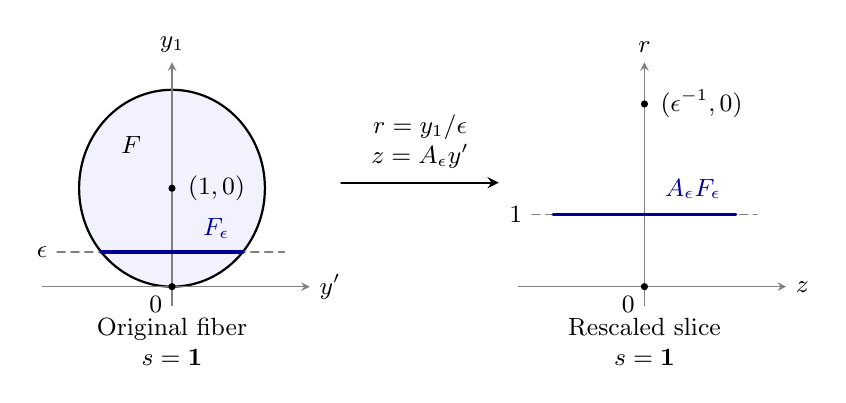
\begin{tikzpicture}[x=1cm,y=1cm,>=stealth,
  every node/.style={font=\small},line cap=round]
  \begin{scope}[shift={(0,0)}]
    \fill[blue!5] (0,1.25) ellipse[x radius=1.18,y radius=1.25];
    \draw[thick] (0,1.25) ellipse[x radius=1.18,y radius=1.25];
    \draw[->,gray] (-1.65,0)--(1.75,0) node[right,black] {$y'$};
    \draw[->,gray] (0,-.24)--(0,2.85) node[above,black] {$y_1$};
    \draw[densely dashed,gray] (-1.46,.44)--(1.43,.44);
    \draw[very thick,blue!60!black] (-.899,.44)--(.899,.44);
    \node[left] at (-1.46,.44) {$\epsilon$};
    \node[anchor=south west,blue!60!black] at (.27,.49) {$F_\epsilon$};
    \fill (0,0) circle[radius=1.3pt];
    \node[below left] at (0,0) {$0$};
    \fill (0,1.25) circle[radius=1.3pt];
    \node[anchor=west] at (.08,1.25) {$(1,0)$};
    \node at (-.52,1.8) {$F$};
    \node[align=center] at (0,-.7) {Original fiber\\$s=\mathbf1$};
  \end{scope}
  \draw[->,thick] (2.15,1.32)--(4.15,1.32);
  \node[align=center] at (3.15,1.84)
    {$r=y_1/\epsilon$\\$z=A_\epsilon y'$};
  \begin{scope}[shift={(6,0)}]
    \draw[->,gray] (-1.6,0)--(1.8,0) node[right,black] {$z$};
    \draw[->,gray] (0,-.24)--(0,2.85) node[above,black] {$r$};
    \draw[densely dashed,gray] (-1.43,.92)--(1.43,.92);
    \draw[very thick,blue!60!black] (-1.16,.92)--(1.16,.92);
    \node[left] at (-1.43,.92) {$1$};
    \node[anchor=south west,blue!60!black] at (.14,.99)
      {$A_\epsilon F_\epsilon$};
    \fill (0,0) circle[radius=1.3pt];
    \node[below left] at (0,0) {$0$};
    \fill (0,2.32) circle[radius=1.3pt];
    \node[anchor=west] at (.08,2.32) {$(\epsilon^{-1},0)$};
    \node[align=center] at (0,-.7) {Rescaled slice\\$s=\mathbf1$};
  \end{scope}
\end{tikzpicture}
\caption{The change from $(y_1,y')$ to $(r,z)$ at the fixed base
point $s=\mathbf1$, shown schematically with one $y'$ coordinate.
The actual fiber need not have the smooth or symmetric shape drawn here.
The slice $y_1=\epsilon$ becomes the slice $r=1$, while
$A_\epsilon$ normalizes its remaining transverse coordinates.
The interior point $(1,0)$ of $F$ is sent to
$(\epsilon^{-1},0)$. The right panel shows only this point, the
origin, and the distinguished slice; the shape of the transformed
fiber is omitted.}
\label{fig:thin-slice}
\end{figure}


Here is a uniform bound for their caps.  Suppose
$(s,r,z)\in C_\epsilon$ with $s_i,r\le T$, where $T\ge1$.
Increase $s$ to $T\mathbf1$ and contract by $1/T$.  This gives
\[
 (\mathbf1,q,z/T)\in C_\epsilon,
 \qquad q=r/T\in[0,1].
\]
The point $(\mathbf1,2,0)$ also belongs to $C_\epsilon$, since
$2\epsilon<1$ and it is obtained by contracting
$(\mathbf1,1,0)\in C$ and then increasing $s$.
Interpolate these two points with weight
\[
 a=\frac1{2-q}\in[1/2,1]
\]
on $(\mathbf1,q,z/T)$.  The resulting point is
$(\mathbf1,1,az/T)$, so the normalized slice gives
\begin{equation}\label{eq:thin-slice-cap-bound}
 |z|\le 4dT\qquad(d>0).
\end{equation}
Equivalently, a slice outer radius $R$ gives the bound $2TR$.
When $d=0$, the bounds on $s$ and $r$ themselves suffice.
Thus caps in the new nonnegative coordinates are uniformly bounded.

Extract a local limit $C_0$ as $\epsilon\downarrow0$, also taking
$c_\epsilon\to c_0$ if $d>0$.  For each fixed $s_i>0$ and $r\ge0$,
the point $(s,r,0)$ belongs to $C_\epsilon$ as soon as
\[
 \epsilon r\le\min\{1,s_1,\ldots,s_k\}.
\]
For $r>0$, this follows by contracting $(\mathbf1,1,0)\in C$
by $\epsilon r$ and then increasing $s$; for $r=0$ it follows
from the original orthant.  Hence $C_0$ contains these points.
Closedness adds all faces with some $s_i=0$, so it contains the
entire nonnegative $(s,r)$ orthant at $z=0$.  The support inequalities
pass to the limit, and \eqref{eq:thin-slice-cap-bound} makes its caps
compact.

For $d>0$, the limit also contains
$\{(\mathbf1,1)\}\times\overline B_1(c_0)$.
The recession argument in Lemma~\ref{lem:model-fibers}, which does
not require full dimension, permits addition of every nonnegative
$(s,r)$ direction.  Thus
\[
 [1,2]^{k+1}\times\overline B_1(c_0)\subset C_0,
\]
which proves full dimension.  For $d=0$, the contained orthant
already has full dimension.  Finally, affine invariance and diagonal
closure of $\mathcal F(D)$ give $C_0\in\mathcal F(D)$.
It is a $(k+1)$-model, contradicting maximality.

This contradiction allowed the initial models, fibers, and
admissible coordinates to vary arbitrarily.  It therefore proves
the uniform assertion \eqref{eq:model-centering}.
Its last conclusion follows, for example, from
\eqref{eq:centered-normalization}.
\end{proof}

We record the quantitative geometric consequence needed for the
later estimates on fixed boxes.

\begin{corollary}\label{cor:normalized-fibers}
Under the hypotheses of Proposition~\ref{prop:centering}, any
chosen positive fiber of any $k$-model can be moved to $s=\mathbf1$
by positive diagonal changes in $s$ and normalized by an invertible
linear change in $y$ so that
\[
 \overline B_{r_0}\subset K_{\mathbf1}
 \subset\overline B_{R_0},
 \qquad r_0=\frac2{C_*+1},\quad R_0=2m.
\]
For every fixed $0<a<1<b$, these normalized models satisfy
\begin{equation}\label{eq:normalized-fiber-box}
 \overline B_{ar_0}\subset K_s
 \subset\overline B_{bR_0}
 \qquad(s\in[a,b]^k).
\end{equation}
Their caps for fixed positive linear forms in $s$ and fixed positive top
levels have uniform bounds, and they contain a fixed interior ball
about $(\mathbf1,0)$.

For any sequence of affine images of $D$ converging to one of these
models, comparable cap and fiber bounds hold eventually, uniformly
on each fixed positive box.  The constants are independent of the
chosen fiber; the required index may depend on its normalization.
For finitely many chosen fibers, one index suffices for all of them.
\end{corollary}

\begin{proof}
The normalization follows from Proposition~\ref{prop:centering}
and Lemma~\ref{lem:linear-normalization}.  Monotonicity and contraction
toward zero give
$aK_{\mathbf1}\subset K_s\subset bK_{\mathbf1}$ on $[a,b]^k$,
proving \eqref{eq:normalized-fiber-box}.
If $\ell(s)=\sum_i a_i s_i$ with $a_i>0$ and $B>0$, put
$T=\max\{1,B/\min_i a_i\}$.  Then
\[
 C\cap\{\ell\le B\}
 \subset [0,T]^k\times\overline B_{TR_0}.
\]
Also $K_s\supset\overline B_{r_0/2}$ whenever each
$s_i\ge1/2$, which supplies the fixed interior ball about
$(\mathbf1,0)$.

Lemma~\ref{lem:cap-compactness} transfers each cap bound to the
approximants; the strict point below its top is the origin.
For a fixed box $[a,b]^k$, a smaller product
$[a,b]^k\times\overline B_{ar_0/2}$ is a compact subset of the
interior of the model, as is seen by first enlarging the positive
$s$ box slightly.  Interior convergence therefore gives the lower
fiber bound on the entire box, and a containing cap gives the upper
bound.  These constants depend only on the displayed fixed
parameters.  Taking the maximum of the finitely many necessary
indices proves the final statement.
\end{proof}
